\par {\color{blue}\textbf{\printdate{2019-7-17}}}
Simple \texttt{2D} impact test were conducted. The geometry is illustrated in Fig. \ref{fig:initgeom}. However, these tests are not running.

\begin{wrapfigure}{R}{0.3\textwidth}
	\centering
	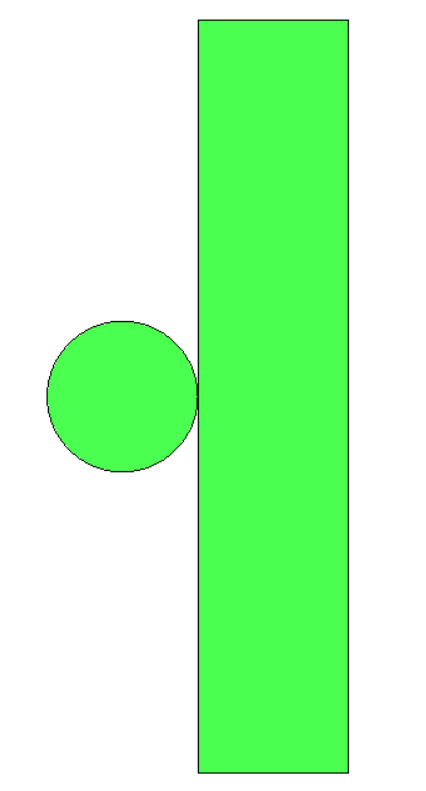
\includegraphics[width=0.3\textwidth]{initial_geometry.PNG}
	\caption{Simple test geometry ('geometry 1').}
	\label{fig:initgeom}
\end{wrapfigure}

\begin{figure}[!h]
	\centering
	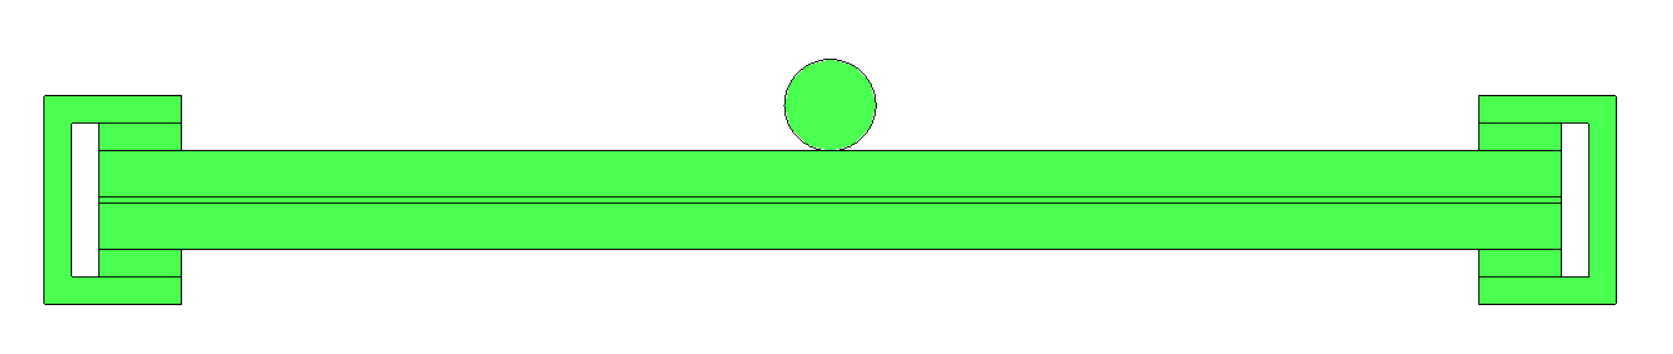
\includegraphics[width=0.8\textwidth]{geometry2.PNG}
	\caption{A more sophisticated test geometry ('geometry 2').}
	\label{fig:geometry2}
\end{figure}

\bigbreak
\noindent{\color{blue}\textbf{\printdate{2019-7-18}}}
Meeting with supervisors. The parameters are wrong,as they need to be determined by use of formulas. For this purpose, it is necessary to introduce additional parameters (bonus parameters), such as total minimum element volume, minimum edge, critical time step of glass, steel, pvb, etc - these do not appear in the program UI. Using the formulas, the simple simulation is now running, provisionally using material for rock (as opposed to glass/steel/pvb).

\bigbreak
\noindent{\color{blue}\textbf{\printdate{2019-7-19}}}
Another geometry is adduced, see Fig. \ref{fig:geometry2}. Simulation using this new geometry, along with proper material data failed. This prompts the following conduction of systematical tests:

\begin{enumerate}[topsep=0pt,itemsep=-1ex,partopsep=1ex,parsep=1ex,label= {\color{blue}\textbf{test\arabic*}\,\,}]
    \item geometry 1, rock
    \item geometry 1, glass/steel
    \item geometry 2, fine mesh, rock
    \item geometry 1, glass
    \item geometry 1, steel
    \item geometry 1, glass, high penalty factor $p$
    \item geometry 1, steel, high penalty factor $p$
    \item geometry 2, fine mesh, glass
    \item geometry 2, fine mesh, steel
    \item geometry 2, fine mesh, pvb
    \item geometry 2, coarse mesh, rock
\end{enumerate}

\textbf{Conclusions from the tests}:

\begin{enumerate}[topsep=0pt,itemsep=-1ex,partopsep=1ex,parsep=1ex,label=\Alph*)]
    \item The issue is not with geometry 1, material rock or material steel.
    \item \textbf{Materials glass and pvb} needs be reconsidered, as tests with these materials have consistently not been successful.
    \item \textbf{Geometry 2} needs to perhaps be reconsidered. The fact that test 11 and test 3 fail implies that some parameters for geometry 2 are wrong.
\end{enumerate}

\bigbreak
{\color{blue}\textbf{\printdate{2019-7-22}}}